	En este capitulo describimos en detalles los pasos que componen la transformación, utilizaremos el modelo ya presentado e introduciremos un modelo 
	PowerDEVS con componentes vectoriales con el fin de ilustrar la transformación de estos componentes.

\section{Modelos DEVS}

        \subsection{Archivos PDS}
        PowerDEVS trabaja principalmente con dos archivos, .PDM y .PDS.
        Los archivos PDM son  por el editor de modelos, pues contiene información estructural, así como información de posición de los modelos dentro del 
        editor, sus parámetros, lo cual indica nombre, tipo y valor, descripción de los modelos, la cantidad de puertos de cada modelo y las conexiones
        entre los modelos, los detalles de cómo esas conexiones son visualizadas por lineas y los detalles del recorrido de esas lineas. 
        Todos estos elementos son utilizados en primera medida con el editor de modelos, pero también son utilizados para generar el archivo PDS el cual es el 
        genera el código de la simulación.
        El archivo PDS contiene información estructural del modelo necesaria para realizar la simulación, en el listado \ref{lst:pdsstruc} se pueden ver un 
        esbozo de su estructura.
        
\todo[inline]{Para seguir una linea lógica mostra el pds del lotka volterra y lo podés relacionar con la figura del modelo 2.5}
\begin{listing}[H]
\begin{minted}{text}
Root-Coordinator
 {
  Simulator
   {
    Path = vector\qss_sum_vec.h
    Parameters = "1","-1","1","0","0","0","0","0",3.000000e+00,"N"
   }
   ...
    Coordinator
     {
      ...
     }
   ...     
  Simulator
   {
        ...
   }
  EIC
   {
   }
  EOC
   {
   }
  IC
   {
        ...
   }
 }
\end{minted}
\caption{Estructura de un archivo PDS.}
\label{lst:pdsstruc}
\end{listing}

        Se puede observar un elemento \texttt{Root-Coordinator} el cual contiene (marcado entre llaves) una lista de \texttt{Simulator}s que representan 
        los modelos atómicos y/o \texttt{Coordinator} que representan los modelos acoplados y tres listas de 
        conexiones \texttt{EIC}, \texttt{EOC} y \texttt{IC}, conexiones de entrada externa (External Input Connections), 
        conexiones de salida externa (external output connections) y conexiones internas (Internal Connections).

        Las lista de conexiones internas (IC) es una lista de par de pares de números naturales, de la forma $(a,b);(c,d)$.
        Donde el primer par se refiere al origen de la conexión (puerto $b$) del modelo $a$ y el segundo al fin de la conexión (puerto $d$) 
        del modelo $c$, ambos modelos se refiere a la lista de modelos (atómicos o acoplados) del actual modelo.
        Es decir el par $(0,0);(1,0)$ indica que el puerto $0$ del segundo modelo (posición 1) está conectado al puerto $0$ del primer modelo.
        \todo[inline]{Acá creo que conectado al puerto 1 del primer modelo. revisar}

        Tanto EIC y EOC siguen el mismo patrón excepto que replazan el modelo de los puertos de salida y entrada respectivamente por $0$. Es decir el elemento 
        $(6,0);(0,1)$ en EOC indica que el puerto $0$ del modelo $6$ (séptima posición)  se encuentra conectado con el puerto $1$ del modelo 
        acoplado, y un par $(0,0);(2,1)$ en EIC indica que el primer puerto (puerto $0$) se encuentra conectado con el modelo $2$ (tercera posición) en su puerto $1$.

        Los modelos acoplados dado que también son modelos DEVS, replican la estructura listado \ref{lst:pdsstruc}.

        Para poder leer esta estructura se cuenta con la librería de PowerDEVS\footnote{http://sourceforge.net/p/powerdevs/code/HEAD/tree/} la cual nos permite acceder
        a la estructura desde C++. 

\section{Modelos Atómicos}
        

\todo[inline]{Acá falta explicar lo más importante antes de arrancar, esto es, que para cada modelo atómico DEVS HAY que escribir un modelo modelica equivalente. Remarcar que esto requiere conocimiento del bloque en sí.}
        Internamente los modelos atómicos son identificados por el parámetro \texttt{Path} en el archivo PDS, para realizar la tradución de este modelo se utiliza 
        un modelo Modelica el cual debe seguir la siguiente especificación:

\begin{itemize}
        \item El código debe ser Modelica ($\mu$-modelica) válido y estar ubicado en el mismo directorio (y nombre del archivo) del código C que el modelo atómico 
        PowerDEVS, con el mismo nombre que el archivo .h, pero con extensión .mo, es decir un modelo con \texttt{vector\textbackslash qss\_sum\_vec.h} 
	utilizará un modelo \texttt{vector/qss\_sum\_vec.h} \footnote{El nombre de los archivos se replaza \quotes{\textbackslash} por \quotes{/} para permitir 
	algunos modelos cuyos \texttt{Path} contiene ese separadores de directorios}
        \item Los parámetros del modelo DEVS deben ser pasado en el parámetro $p$
        \item Los valores de entrada del modelo son asociados a la variable $u$
        \item Los valores de salida del modelos son asociados a la variable $y$
\end{itemize}

\todo[inline]{falta explicar que las variables de entrada y salida van a ser arreglos para representar los distintos puertos de entrada/salida}
\todo[inline]{Lo mismo para p, decir que es un arreglo porque un bloque puede tener muchos (hasta 10) parámetros}

\todo[inline]{el ejemplo del integrado está bien pero yo antes mencionaría cuántos puertos de entrada/salida tiene, cuales son sus parámetros y qué relación tiene su entrada con su salida. recién ahi mostrar el codigo}


        Por ejemplo el código del integrador, originalmente ubicado en el archivo qss\_integrator.h de PowerDEVS, se ubica en el archivo qss\_integrator.mo 
	mostrado en el listado \ref{lst:qssintegrator.mo} ambos dentro del directorio qss.

\begin{listing}[H]
\begin{minted}{modelica}
class QSSIntegrator
  parameter Real p[4]={0,0,0,0,0,0,0,0};
  parameter Real x0 = p[4];
  Real u[1];
  Real y[1](start = {x0});
equation
  der(y[1]) = u[1];
end QSSIntegrator;
\end{minted}
\caption{Modelo qss\_integrator.mo}
\label{lst:qssintegrator.mo}
\end{listing}

        El modelo Lotka Volterra cuenta con dos integradores (con los mismo parámetros) representados en el listado \ref{lst:qssint.pds}, en este se puede ver 
        el valores de \texttt{Path} y \texttt{Parameters} que componen todos los modelos atómicos (por supuesto con los valores diferentes).

\begin{listing}[H]
\begin{minted}{text}
  ...
  Simulator
   {
    Path = qss/qss_integrator.h
    Parameters = "QSS3","1e-6","1e-3","0.5"
   }
   ...
\end{minted}
\label{lst:qssint.pds}
\caption{Extracto del modelo Lotka Volterra, modelo atómico de un integrator.}
\end{listing}

        Luego de remplazar los parámetros en la variable \texttt{p}, se prefijan todas las variables del modelo\footnote{La única variable que no se prefijada 
        es \texttt{time}} por el nombre del modelo y su posición en este caso con el prefijo 
        \quotes{\texttt{QSSIntegrator\_1\_}}, de esta forma podremos combinar varios modelos atómicos de forma que no existan \quotes{colisión} de nombres de variables,
        es decir dos variables de distintos modelos atómicos con el mismo nombre en Modelica. 

\begin{listing}[H]
\begin{minted}{modelica}
class QSSIntegrator
  parameter Real QSSIntegrator_1_p[4]={0,1e-6, 1e-3, 0.5};
  parameter Real QSSIntegrator_1_x0 = p[4];
  Real QSSIntegrator_1_u[1];
  Real QSSIntegrator_1_y[1](start = {QSSIntegrator_1_x0});
equation
  der(QSSIntegrator_1_y[1]) = QSSIntegrator_1_u[1];
end QSSIntegrator;
\end{minted}
\caption{Transformación parcial de un modelo atómico de un integrator en el modelo de ejemplo Lotka Volterra.}
\end{listing}

        Los parámetros son remplazados en el modelo, evaluándolos en Scilab\footnote{Para realizar la evaluación en Scilab se utiliza el mismo mecanismo que 
        provee (y utiliza) PowerDEVS.}, lo que los transforma en float, los cuales son presentados como reales (\texttt{Real}) en el código.

\todo[inline]{Qué implciacia tiene esto? Porqué se puede ignorar un modelo? Qué pasa con las conexiones desde/hacia él?}
        Los modelos (atómicos) no encontrados son ignorados en la traducción y se reportan en el registro (archivo .log) de la conversión.

        Esta transformación se repite para todos los modelos atómicos del archivo .PDS dentro del \texttt{Root-Coordinator}, los modelos acoplados 
        (dentro de un \texttt{Coordinator}) deben ser transformados a un conjunto de atómicos equivalentes \quotes{Plano}, mediante la transformación
	descripta en la siguiente sección.

\section{Modelos Acoplados Planos}

        Llamamos \emph{Modelos Acoplados Planos} a los Modelos que sólo contienen \emph{Modelos Atómicos}. Es decir que no contienen Modelos acoplados.

        Cada uno de los modelos atómicos que incluye se transforma de la misma forma que describimos en la sección anterior y dado que no existen \quotes{colisiones} 
        de nombres variables, podemos combinar las diferentes secciones en un modelo compuesto el cual tendrá todas las secciones \texttt{equation}, 
	\texttt{initial equation} y declaraciones de cada uno de los modelos.
        Luego cada conexión entre Modelos Atómicos es replicada en el código de Modelica resultante. Los modelos Atómicos cuyo entrada (o salida) 
	son escalares son conectados con un ecuación del tipo $u = y$ mientras que los modelos vectoriales son conectados con la misma ecuación, 
	solo que dentro de un \texttt{for}, el cual itera sobre su dimensión.

\begin{listing}[H]
        \inputminted[linenos]{modelica}{src/lotka_volterra-orig.mo}
        \caption{Modelo Lotka Volterra convertido de PowerDEVS a $\mu$-Modelica}
        \label{lst:lotka_volterra-orig.mo}
\end{listing}

        En el listado \ref{lst:lotka_volterra-orig.mo} se puede ver el resultado de la conversión del modelo Lotka Volterra, en el se puede apreciar en las líneas 
        2 a 21 correspondientes a las declaraciones de las variables de los modelos atómicos y de las líneas 22 a 27 correspondientes a las ecuaciones de estos 
        modelos y de la línea 28 a 35 son las ecuaciones correspondientes a las conexiones entre modelos atómicos.

        En las lineas de conexiones (lineas 28 a 35) se puede ver cómo se utilizan las variables \texttt{u} e \texttt{y} (prefijadas con sus correspondientes nombres 
	de modelos atómicos y posición). Tanto los puertos de entrada, \texttt{u}, como los puertos de salida, \texttt{y}, son representados en Modelica como arreglos,
        permitiendo a modelos que cuentan con más de un puerto reflejar este hecho, asociando cada puerto con la posición correspondiente del arreglo. 
        Cabe mencionar que existe un desfase, ya que los puerto en PowerDEVS son enumerados desde el cero, mientras que Modelica inician los arreglos en uno, por lo
        que el puerto \texttt{n} corresponde a la variable \texttt{u[n+1]} si es un puerto de entrada y \texttt{y[n+1]} si es un puerto de salida.

        En el ejemplo Lotka Volterra no hay modelos atómicos vectoriales, veremos más adelante un ejemplo vectorial, pero es oportuno mencionar que los modelos
        vectoriales difieren en la forma en que se conectan, dado que la conexión debe realizarse iterando, con un \texttt{for}, sobre la primera dimensión del 
        arreglo que representa el puerto. En el caso escalar, que es el caso por omisión, sólo alcanza con igualar las variables mencionadas.


\section{Modelos Acoplados Jerárquicos} \label{aplanado}
        En la sección anterior mostramos cómo son convertidos modelos acoplados planos, para convertir un modelo acoplado jerárquico, es decir un modelos con más 
        modelos acoplados internos, vamos a generar un modelo acoplado plano, equivalente al modelo jerárquico inicial.

        Para realizar el aplanado, se recorre recursivamente los modelos acoplados:

        \begin{itemize}
                \item por cada modelo acoplado si solo tiene modelos atómicos, es remplazado por los modelos atómicos internos, los cuales se encuentran conectados 
                        sin modificaciones excepto por las conexiones externas, las cuales son reasignadas de forma de mantener las conexiones.
                \item si el modelo acoplado contiene otros modelos acoplados entonces aplanamos ese modelo recursivamente.
        \end{itemize} 

        De esta forma obtenemos un modelo con solo modelos atómicos el cual podemos convertir con el procedimiento anteriormente descripto.

\begin{figure}[H]
        \begin{minipage}{0.5\textwidth}
        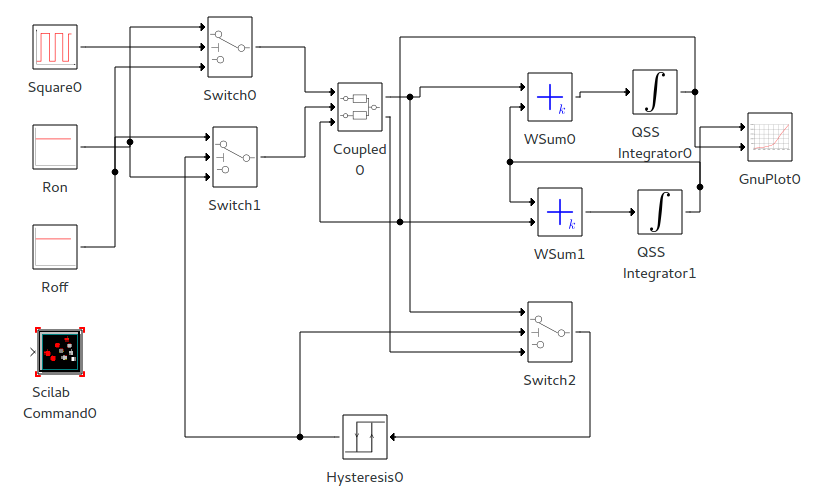
\includegraphics[width=\linewidth]{buck_disk}
        \end{minipage}
        \begin{minipage}{0.5\textwidth}
        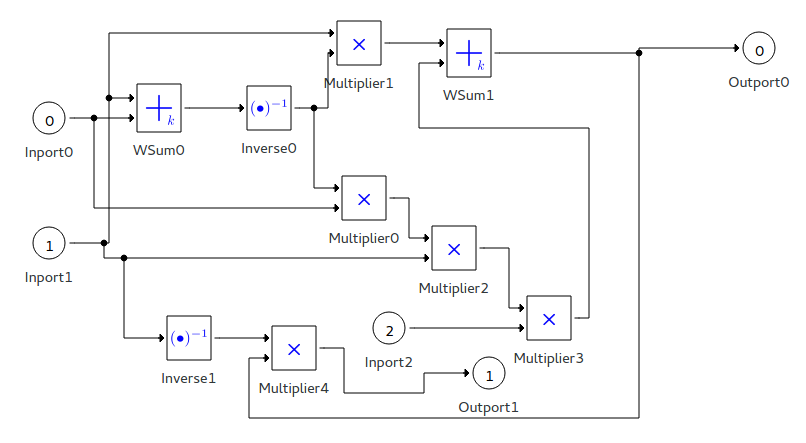
\includegraphics[width=\linewidth]{buck_disk_coupled0}
        \end{minipage}
 \label{fig:coupledsample}
 \caption{Ejemplo de Modelo acoplado(derecha), junto a una detalle del modelo \texttt{Coupled0}}
\end{figure}

        En la figura \ref{fig:coupledsample}  se observa a la derecha el modelo de un convertidor de potencia, el cual introduciremos con mayores
	 detalles en una sección posterior, y a la izquierda el modelo acoplado \texttt{Coupled0}.

\todo[inline]{Esta figura está perfecta pero yo agregaría a cada modelo qué numero de hijo es dentro de su acoplado padre. así queda más claro lo de las conexiones después}
\begin{figure}[H]

  %\setcapwidth{0.6\textwidth}
  \makebox[\textwidth][c]{%
        \begin{minipage}[t][][b]{.59\textwidth}
        \begin{tikzpicture}[%
          grow via three points={one child at (0.5,-0.7) and
          two children at (0.5,-0.7) and (0.5,-1.4)},
          edge from parent path={(\tikzparentnode.south) |- (\tikzchildnode.west)}]
          \node {Root-Coordinator}
            child { node {Scilab Command0}}             
            child { node {QSS Integartor0}}
            child { node {QSS Integartor1}}             
            child { node {Coupled0}
              child { node {WSum0}}
              child { node {Inseverse0}}
              child { node {Multiplier0}}
              child { node {Multiplier1}}
              child { node {Multiplier2}}
              child { node {Inseverse1}}
              child { node {Multiplier3}}
              child { node {Multiplier4}}
              child { node {WSum1}}
            }
            child [missing] {}                          
            child [missing] {}                          
            child [missing] {}                          
            child [missing] {}                          
            child [missing] {}                          
            child [missing] {}                          
            child [missing] {}                          
            child [missing] {}                          
            child [missing] {}                          
            child { node {Switch0}}
            child { node {Ron}}
            child { node {Roff}}
            child { node {Square0}}
            child { node {GNUPlot0}}
            child { node {Hysteresis0}}
            child { node {Switch1}}
            child { node {WSum0}}
            child { node {WSum1}};
        \end{tikzpicture}
        \end{minipage} %
        \hfill
        \begin{minipage}[t][][b]{.59\textwidth}
        \begin{tikzpicture}[%
          grow via three points={one child at (0.5,-0.7) and
          two children at (0.5,-0.7) and (0.5,-1.4)},
          edge from parent path={(\tikzparentnode.south) |- (\tikzchildnode.west)}]
          \node {Root-Coordinator}
            child { node {Scilab Command0}}             
            child { node {QSS Integartor0}}
            child { node {QSS Integartor1}}             
            child { node {WSum0}}
            child { node {Inseverse0}}
            child { node {Multiplier0}}
            child { node {Multiplier1}}
            child { node {Multiplier2}}
            child { node {Inseverse1}}
            child { node {Multiplier3}}
            child { node {Multiplier4}}
            child { node {WSum1}}
            child { node {Switch0}}
            child { node {Ron}}
            child { node {Roff}}
            child { node {Square0}}
            child { node {GNUPlot0}}
            child { node {Hysteresis0}}
            child { node {Switch1}}
            child { node {WSum0}}
            child { node {WSum1}};
        \end{tikzpicture}
        \end{minipage}%
}       
        \caption{Modelo convertidor Buck de potencia, jerarquía original (izquierda) y aplanada (derecha)}
        \label{fig:coupled-tree}
\end{figure}

	En la figura \ref{fig:coupled-tree} se puede observar la forma en que se modifican las jerarquía, esencialmente se mueven los modelos atómicos 
        a la jerarquía superior y se modifican las conexiones de forma que se mantengan los enlaces, es decir todas las conexiones entre modelos atómicos 
        listados despues del modelo acoplado deben ser ajustados para tomar en cuenta los nuevos modelos atómicos agregados.
\todo[inline]{En realidad para tener en cuenta que ahora tienen otro número de modelo. aclararlo}

\begin{listing}
\begin{minipage}[t]{0.5\linewidth}
\centering
\begin{minted}[linenos]{text}
 IC
   {
   (13,0);(1,0)
    (12,0);(2,0)
    (8,0);(4,1)
    (4,0);(3,0)
    (5,0);(3,1)
    (3,1);(11,2)
    (11,0);(10,0)
    (2,0);(9,0)
    (2,0);(12,0)
    (2,0);(13,1)
    (3,0);(11,0)
    (3,0);(13,0)
    (10,0);(11,1)
    (10,0);(5,1)
    (1,0);(3,2)
    (1,0);(12,1)
    (1,0);(9,1)
    (6,0);(5,2)
    (6,0);(4,0)
    (7,0);(5,0)
    (7,0);(4,2)
}
\end{minted}
\end{minipage}
\begin{minipage}[t]{0.5\linewidth}
\begin{minted}[linenos]{text}
     EIC
       {
        (0,2);(4,1)
        (0,0);(2,1)
        (0,0);(0,1)
        (0,1);(3,1)
        (0,1);(5,0)
        (0,1);(7,0)
        (0,1);(0,0)
       }
      EOC
       {
        (6,0);(0,1)
        (8,0);(0,0)
       }
      IC
       {
        (0,0);(1,0)
        (7,0);(8,0)
        (2,0);(3,0)
        (3,0);(4,0)
        (5,0);(6,0)
        (4,0);(8,1)
        (1,0);(2,0)
        (1,0);(7,1)
        (8,0);(6,1)
       }
\end{minted}
\end{minipage}
\label{lst:connections}
\caption{Conexiones del modelo acoplado convertidor Buck de potencia, a la derecha, las conexiones del primera nivel (\texttt{Root Coordinator}), a la derecha, 
        las conexiones, external entrada (EIC) y salida (EOC) y las conexiones internas (IC) del modelo acoplado (\texttt{Coupled0}).}
\end{listing}

        En el modelo aplanado, se modificarán del listado \ref{lst:connections} las conexiones de forma que se respeten las conexiones entre los modelos atómicos, 
	si pasan por un puerto de salida o de entrada, vemos tres tipos de conexiones que deben ser modificadas:

\begin{itemize}
        \item Conexiones que involucran modelos atómicos ubicados después del modelo acoplado y no están relacionadas con el modelo acoplado, 
        estas conexiones deben ser modificadas dado que insertaremos los modelos atómicos del modelo acoplado que estamos aplanando, y los modelos 
        ubicados después del modelo acoplado serán desplazados.
        
\begin{listing}[H]
        \begin{minipage}{0.5\textwidth}
\begin{minted}[linenos]{text}
      IC
        {
         (13,0);(1,0)
         (12,0);(2,0)
         (8,0);(4,1)
         (11,0);(10,0)
         (2,0);(9,0)
         (2,0);(12,0)
         (2,0);(13,1)
         (10,0);(11,1)
         (10,0);(5,1)
         (1,0);(12,1)
         (1,0);(9,1)
         (6,0);(5,2)
         (6,0);(4,0)
         (7,0);(5,0)
         (7,0);(4,2)
        }
\end{minted}
        \end{minipage}
        \begin{minipage}{0.5\textwidth}
\begin{minted}[linenos]{text}
      IC
        {
         (21,0);(1,0)
         (20,0);(2,0)
         (16,0);(12,1)
         (19,0);(18,0)
         (2,0);(17,0)
         (2,0);(20,0)
         (2,0);(21,1)
         (18,0);(19,1)
         (18,0);(13,1)
         (1,0);(20,1)
         (1,0);(17,1)
         (14,0);(13,2)
         (14,0);(12,0)
         (15,0);(13,0)
         (15,0);(12,2)
       }
\end{minted}
        \end{minipage}
\label{lst:conexiones1}
\caption{Conexiones internas, como se encontraban originalmente a la izquierda y modificadas a la derecha}
\end{listing}

        En el listado \ref{lst:conexiones1} se puede ver a la derecha las conexiones que fueron afectadas y a la izquierda como fueron afectadas, en nuestro ejemplo
        se sumo $8$ (ya que insertaremos esa cantidad de modelos) a los modelos mayores que $3$ (ya que el modelos acoplado que estamos aplanando se encuentra en 
        es posición).

        \item Agregamos las conexiones internas del modelo acoplado que eliminaremos al modelo acoplado \texttt{Root-Coordinator}, estas conexiones deben ser 
        modificadas ya que los modelos atómicos insertados son insertados en la posición del modelo acoplado eliminado.

\begin{listing}
\begin{minipage}[t]{0.5\textwidth}
\begin{minted}{text}
      IC
       {
        (0,0);(1,0)
        (7,0);(8,0)
        (2,0);(3,0)
        (3,0);(4,0)
        (5,0);(6,0)
        (4,0);(8,1)
        (1,0);(2,0)
        (1,0);(7,1)
        (8,0);(6,1)
       }
\end{minted}
        \end{minipage}
        \begin{minipage}[t]{0.5\textwidth}
\begin{minted}{text}
      IC
       {
        (3,0);(4,0)
        (10,0);(11,0)
        (5,0);(6,0)
        (6,0);(7,0)
        (8,0);(9,0)
        (7,0);(11,1)
        (4,0);(5,0)
        (4,0);(10,1)
        (11,0);(9,1)
       }
\end{minted}
        \end{minipage}
        \label{lst:conexiones2}
        \caption{Conexiones internas del modelo acoplado a eliminar, a la izquierda como aparecen originalmente, a la derecha como serán insertados}
\end{listing}

        En el listado \ref{lst:conexiones2} se pueden ver las conexiones como se encontraban originalmente (izquierda) y como serán insertadas (derecha)
        estas son el resultados de desplazar los modelos, en nuestro ejemplo $3$ posiciones, por lo que sumamos ese desplazamiento a los modelos.

\begin{figure}[!htbp]
\centering
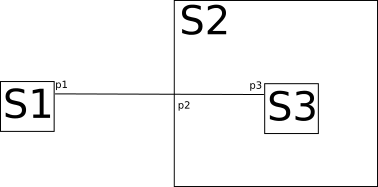
\includegraphics[width=.75\textwidth]{text3418}
\label{fig:aplanado-ports}
\caption{Esquema de conexiones, el modelo \texttt{S1} y \texttt{S3} son modelo atómico, \texttt{S2} es el modelo acoplado que estamo aplanando.\
	\texttt{S1} y \texttt{S2} están conectados a travéz de los puertos \texttt{p1} y \texttt{p2} respectivamente. Luego, el modelo \texttt{S3} conecta con
	el exterior a travéz del modelo acoplado que lo contiene por el puerto \texttt{p2} y el puerto  \texttt{p3}.
	}
\end{figure}

	Se puede ver en la figura \ref{fig:aplanado-ports} un esquema de conexiones, donde el modelo $S2$ es un modelo acoplado que contiene el modelo $S3$.
	 El modelo atómico $S1$ se conecta a travéz del puerto $p2$.
	 Entonces si consideramos que $p2$ es un puerto de entrada externa, veremos las siguientes conexiones:

	\begin{itemize}
	\item IC : \texttt{(S1,p1);(S2,p2)}
	\item EIC : \texttt{(0,p2);(S3,p3)}
	\end{itemize}

	entonces la conexiones en el modelo aplanado es \texttt{($S1$,$p1$);($S3$,$p3$)} y $S1$ debe ser desplazado según la cantidad de modelos que contiene $S2$ y 
	$S3$ deberá ser desplazado segun la posición de $S2$.

	Si consideramos que $p2$ es un puerto de salida las conexiones serán:

	\begin{itemize}
	\item IC : \texttt{(S2,p2);(S1,p1)}
	\item EOC : \texttt{(S3,p3);(0,p2)}
	\end{itemize}

	entonces la conexiones en el modelo aplanado es \texttt{($S3$,$p3$);($S1$,$p1$)} e igual que en el caso anterior, $S1$ debe ser desplazado segun la 
	cantidad de modelos que contiene $S2$ y $S3$ deberá ser desplazado según la posición de $S2$.


\begin{listing}
\begin{minipage}[t]{0.3\linewidth}
\begin{minted}{text}
      IC
       {
        (3,1);(11,2)
        (3,0);(11,0)
        (3,0);(13,0)
       }
\end{minted}
\end{minipage}
\begin{minipage}[t]{0.3\linewidth}
\begin{minted}{text}
      EOC
       {
        (6,0);(0,1)
        (8,0);(0,0)
       }
\end{minted}
\end{minipage}
\begin{minipage}[t]{0.3\linewidth}
\begin{minted}{text}
      IC
       {
        (9,0);(19,2)
        (11,0);(19,0)
        (11,0);(21,0)
       }
\end{minted}
\end{minipage}
\label{lst:conexiones3}
\caption{Conexiones internas desde el modelo acoplado hacia otro modelo (izquierda), conexiones externas de salida (centro), conexiones internas a agregar al modelo aplanando(derecha).}
\end{listing}

\begin{listing}
\begin{minipage}[t]{0.3\linewidth}
\begin{minted}{text}
      IC
       {
        (4,0);(3,0)
        (5,0);(3,1)
        (1,0);(3,2)
       }
\end{minted}
\end{minipage}
\begin{minipage}[t]{0.3\linewidth}
\begin{minted}{text}
      EIC
       {
        (0,2);(4,1)
        (0,0);(2,1)
        (0,0);(0,1)
        (0,1);(3,1)
        (0,1);(5,0)
        (0,1);(7,0)
        (0,1);(0,0)
       }
\end{minted}
\end{minipage}
\begin{minipage}[t]{0.3\linewidth}
\begin{minted}{text}
      IC
       {
        (12,0);(5,1)
        (12,0);(3,1)
        (13,0);(6,1)
        (13,0);(8,0)
        (13,0);(10,0)
        (13,0);(3,0)
        (1,0);(7,1)
       }
\end{minted}
\end{minipage}
\label{lst:conexiones3}
\caption{Conexiones internas hacia el modelo acoplado (izquierda), conexiones externas de entrada(centro), conexiones internas a agregar al modelo aplanando(derecha).}
\end{listing}
\end{itemize}

	Agregando estas conexiones se elimina el modelo acoplado y se preserva las conexiones, y recorriendo el esquema jerárquico de modelos en profundidad, 
	aplanando los modelos acoplado más profundos primero, podemos utiliza el algoritmo de forma de aplanar el modelo más profundo únicamente.

\section{Modelos Vectoriales}
	Como ya mencionamos, los modelos vectoriales son modelos atómicos en el cual las entradas y/o salidas son vectoriales. En los modelos Modelica, 
	las variables \texttt{u} e \texttt{y} representan los puertos de entrada y salida respectivamente, por lo que serán del tipo arreglo de arreglos de reales,
	mientras que en los modelos atómicos no vectoriales (escalares) tienen variables que representan los puertos de entrada y salida como arreglos de reales. 

	En el momento cuando las estructura del modelo acoplado es transformada a Modelica, es decir cuando se agregan las ecuaciones de igualdad entre las
	variables de entrada y salida de diferentes modelos, según lo dispongan la estructura del modelo, es decir las conexiones internas, en PowerDEVS 
	no existe una forma de determinar si un modelo es vectorial o no, por lo que debemos indicarlo dentro del modelo Modelica, ya que si no lo hacemos 
	agregaremos una ecuación que iguala un arreglo con una entrada de un arreglo, para prevenir este problema los modelos vectoriales deben indicarse 
	con la anotación (\texttt{annotation}) de Modelica $PD2MO$, por ejemplo:

\begin{itemize}
	\item \texttt{annotation(PD2MO = \{Scalar, Scalar\});} entrada y salida son escalares, este es el caso por omisión y no es necesario declararlo.
	\item \texttt{annotation(PD2MO = \{Scalar, Vector\});} entrada escalar y salida vectorial
	\item \texttt{annotation(PD2MO = \{Vector, Scalar\});} entrada escalar y salida vectorial
	\item \texttt{annotation(PD2MO = \{Vector, Vector\});} entrada y salida vectoriales.
\end{itemize}

	De esta forma podemos realizar la conexiones correctamente y generar un error en caso de encontrar una conexión escalar con una vectorial. 

\section{Transformaciones Extras}
	
	Existen dos tipos de transformaciones extras que deben ser aplicadas con el fin de que el código generado sea $\mu$-Modelica, en particular 
	estas transformaciones se agrupan en dos:
	\begin{itemize}
	\item Causalización de variables, este es un programa descripto en \cite{Mod15}
	\item Transformaciones de Modelica a $\mu$-Modelica, si bien existe un programa con esta finalidad, éste no implementa (al momento de escribir este texto)
	las transformaciones que necesitamos por lo que son descriptas en la sección \ref{sec:transform}.
	\end{itemize}
